% ============================================================================
% IV. EXPERIMENTAL SETUP (REVISED - FINAL WITH BOTH FIGURES)
% ============================================================================
\section{Experimental Setup}
\label{sec:experimental_setup}

% ----------------------------------------------------------------------------
\subsection{Datasets}
\label{sec:datasets}

To evaluate the framework's generalizability beyond a single specimen type, three distinct ME-HSI datasets were used.
The Lichens dataset, with four expert-annotated morphological classes, served as the primary supervised benchmark.
The Collagen Sponges dataset, with three crosslinker concentration classes, tested transferability to a chemically distinct sample family.
The Drop Data dataset, with no labels at all, provided a blind validation case: the framework was applied without any reference signal and evaluated post-hoc against a ground truth derived from unsupervised clustering of the full spectral cube.
This three-dataset design directly addresses the joint concerns of dataset breadth and the rigor of the unsupervised claim.

% ----------------------------------------------------------------------------
\subsubsection{Lichens Dataset (Primary, Supervised)}
\label{sec:dataset_lichens}

The primary dataset comprised ME-HSI acquisitions of lichen specimens---composite organisms formed by symbiotic associations between fungi and photosynthetic partners (algae or cyanobacteria).
Lichens serve as important bioindicators for environmental monitoring, and their autofluorescence signatures reflect both fungal and algal components~\cite{meysurova2021optical}.

\begin{table}[!t]
\centering
\caption{Lichen Dataset Specifications}
\label{tab:dataset}
\begin{tabular}{@{}ll@{}}
\toprule
\textbf{Parameter} & \textbf{Value} \\
\midrule
Spatial dimensions & $1040 \times 925$ pixels \\
Excitation wavelengths & 8 (310, 325, 340, 365, 385, 400, 415, 430\,nm) \\
Emission range & 420--720\,nm \\
Emission bands (per ex.) & 22--28 (variable after Rayleigh cutoff) \\
Total EEM pairs & 192 \\
Spectral resolution & $\sim$12.5\,nm \\
Ground-truth classes & 4 distinct classes \\
\bottomrule
\end{tabular}
\end{table}

Table~\ref{tab:dataset} summarizes the dataset details.
The acquisition system employed an LED-based multi-excitation source (WheeLED, Mightex, Toronto, CA) spanning the 310 - 440\,nm range. Images were acquired with a Nuance FX hyperspectral camera (PerkinElmer, Waltham, MA), capturing emission spectra from 420 to 720\,nm with 10\,nm step at each excitation.
Exposure times and LED power were recorded for intensity normalization per Equation~\eqref{eq:normalization}.

Ground-truth annotations were generated based on the knowledge of the origins of each lichen species obtained from the Takhtajyan Institute of Botany, National Academy of Sciences of Armenia.
Four regions were delineated, providing ground-truth annotations for supervised evaluation.
The total of 192 valid excitation-emission pairs results from variable emission windows after first- and second-order Rayleigh scattering removal (Section~\ref{sec:preprocessing}).

% ----------------------------------------------------------------------------
\subsubsection{Collagen Sponges Dataset (Secondary, Supervised)}
\label{sec:dataset_pepsin}

The Collagen Sponges dataset comprised ME-HSI acquisitions of collagen sponges samples prepared at three distinct crosslinker concentrations.
Collagen autofluorescence in the near-UV/blue range is a well-established structural biomarker, and crosslinker concentration directly modulates the supramolecular organization of collagen fibrils, producing measurable shifts in both emission peak position and intensity~\cite{lakowicz2006principles,meysurova2021optical}.
This dataset tests whether the framework, tuned on lichen biology, transfers to a chemically distinct fluorophore family without modification.

\begin{table}[!t]
\centering
\caption{Collagen Sponges Dataset Specifications}
\label{tab:dataset_pepsin}
\begin{tabular}{@{}ll@{}}
\toprule
\textbf{Parameter} & \textbf{Value} \\
\midrule
Spatial dimensions & $\sim$$1040 \times 925$ pixels (sample-dependent) \\
Excitation wavelengths & 6 (310, 325, 340, 365, 385, 400\,nm) \\
Emission range & 420--720\,nm \\
Emission bands (per ex.) & 22--28 (variable after Rayleigh cutoff) \\
Total EEM pairs & 158 \\
Spectral resolution & 10\,nm \\
Ground-truth classes & 3 crosslinker concentrations \\
Annotated pixels & 39,970 \\
\bottomrule
\end{tabular}
\end{table}

Table~\ref{tab:dataset_pepsin} summarizes the specifications.
Compared to the Lichens dataset, this acquisition uses fewer excitation channels (6 vs.\ 8) because the longer-UV excitations (415 and 430\,nm) added negligible discriminative signal in preliminary tests on these samples.
The resulting 158 valid EEM pairs constitute a different spectral coverage than the Lichens benchmark, so the wavelength selection task is genuinely new rather than a re-run on the same grid.

% ----------------------------------------------------------------------------
\subsubsection{Drop Data Dataset (Blind, Unsupervised)}
\label{sec:dataset_drops}

The Drop Data dataset was acquired specifically to stress-test the unsupervised claim of the framework.
Sixteen fluorescent drops of varied composition were deposited onto a stage in a $4 \times 7$ grid (28 wells; 12 wells empty or below detection threshold) and imaged at seven excitation wavelengths without any reference labeling, classification scheme, or ground-truth annotation.
Crucially, no labels of any kind were available during selection, and the framework was applied identically to how it would be deployed on a previously-unseen acquisition.
A post-hoc ground truth, used only for evaluation, was constructed by Ward hierarchical clustering of the full 214-dimensional drop-mean spectra; this analysis revealed three distinct spectral archetypes (3 ``bright'' drops, 5 ``moderate'' drops, and 8 ``baseline'' drops), denoted Types~0, 1, and 2 in this paper.

\begin{table}[!t]
\centering
\caption{Drop Data Dataset Specifications}
\label{tab:dataset_drops}
\begin{tabular}{@{}ll@{}}
\toprule
\textbf{Parameter} & \textbf{Value} \\
\midrule
Spatial dimensions (cropped) & $175 \times 348$ pixels \\
Excitation wavelengths & 7 (310, 325, 340, 365, 385, 400, 415\,nm) \\
Emission range & 420--720\,nm \\
Emission bands (per ex.) & 29--31 (variable after Rayleigh cutoff) \\
Total EEM pairs & 214 \\
Spectral resolution & 10\,nm \\
Reference cubes & 1 Background + 1 Whitelight \\
Specimen drops & 16 (post-crop, post-detection) \\
Spectral archetypes (Ward, $k=3$) & 3 (post-hoc, evaluation only) \\
\bottomrule
\end{tabular}
\end{table}

Table~\ref{tab:dataset_drops} summarizes the specifications.
A bottom-of-image region containing a calibration ruler was excluded by cropping at row 175 of the original $256 \times 348$ acquisition.
Acquisition used HDR bracketing with 2--3 integration times per excitation to handle the wide intra-scene dynamic range; the longest non-saturating exposure was selected per excitation for analysis.
The Background cube was used for dark-frame subtraction; the Whitelight cube was inspected but not used as a divisor because it contained the ruler rather than a clean flat-field reference.

For this dataset, every numerical comparison in Section~\ref{sec:results} between the proposed method and the eight baseline methods is computed without any label information entering the selection pipeline.
The KNN evaluation metric uses the post-hoc Ward types only as outcome labels for scoring---never as inputs to the selection step.

% ----------------------------------------------------------------------------
% Figure: RGB composite of lichen samples
% ----------------------------------------------------------------------------
\begin{figure}[!t]
\centering
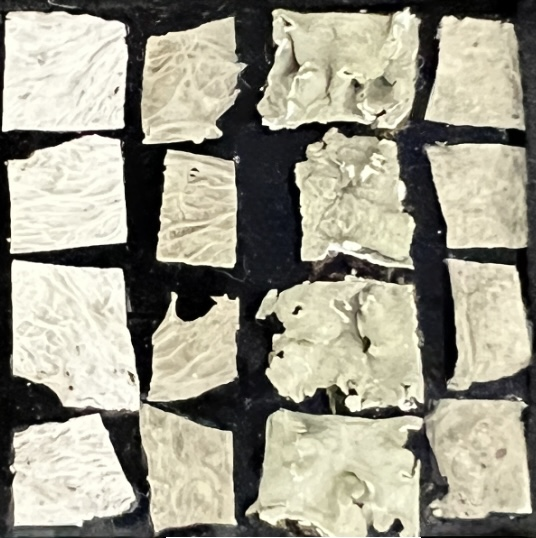
\includegraphics[width=0.45\textwidth]{paper/figures/LichensRGB.jpg}
\caption{Visual appearance of lichens used in this study. The first two columns are ~7x7mm pieces of Ramalina Sinesis (back and front). The third and fourth columns are Flavopunctelia Soredica and Ramalina Fraxinea, respectively (both front surfaces). }
\label{fig:lichen_rgb}
\end{figure}

% ----------------------------------------------------------------------------
% Figure: ROI Overlay showing ground-truth and validation regions
% ----------------------------------------------------------------------------
\begin{figure}[!t]
\centering
\includegraphics[width=0.48\textwidth]{paper/figures/LichensLabels and ROI.png}
\caption{Ground-truth annotation and baseline classification results using all 192 bands. The 16 lichen specimens are arranged in a $4 \times 4$ grid, with columns corresponding to the four classes. Equal-sized square ROIs (one per class, $50 \times 60$ pixels each) in the first row provide training exemplars for KNN evaluation. These ROIs were used \emph{only} for post-hoc validation of wavelength selection quality; they did not influence the unsupervised selection pipeline.}
\label{fig:roi_overlay}
\end{figure}

% ----------------------------------------------------------------------------
\subsection{Implementation Details}
\label{sec:implementation}

The framework was implemented in Python 3.10 using PyTorch 2.0~\cite{paszke2019pytorch} for deep learning components and scikit-learn 1.3~\cite{pedregosa2011scikit} for classification and metrics.
All experiments were conducted on a workstation with an NVIDIA RTX 4070 GPU (8\,GB VRAM) and 64\,GB system RAM.

\subsubsection{Autoencoder Hyperparameters}
Table~\ref{tab:hyperparams} lists the autoencoder configuration.
$k_1 = k_3 = 20$ filters were employed based on preliminary experiments showing this provided sufficient capacity without overfitting.
The $5 \times 5$ spatial filter captured local texture patterns relevant for biological specimens.
Sigmoid activations ensured outputs remained in $[0, 1]$, matching the normalized input range.

\begin{table}[!t]
\centering
\caption{Autoencoder Hyperparameters}
\label{tab:hyperparams}
\begin{tabular}{@{}lll@{}}
\toprule
\textbf{Parameter} & \textbf{Value} & \textbf{Rationale} \\
\midrule
Encoder filters ($k_1$) & 20 & Capacity vs.~complexity \\
Latent filters ($k_3$) & 20 & Bottleneck dimensionality \\
Spatial filter size & $5 \times 5$ & Local pattern capture \\
Spectral filter size & min(5, $N_{\text{em}}$) & Variable band counts \\
Activation & Sigmoid & Match $[0,1]$ input \\
Dropout rate & 0.5 & Regularization \\
Patch size & $64 \times 64$ & GPU memory constraints \\
Patch overlap & 8 pixels & Boundary continuity \\
Batch size & 32 & Training stability \\
Optimizer & Adam~\cite{kingma2014adam} & Adaptive learning rates \\
Initial learning rate & 0.001 & Standard default \\
LR scheduler & ReduceOnPlateau & Convergence refinement \\
LR factor & 0.5 & Reduction magnitude \\
Patience (LR) & 5 epochs & Schedule sensitivity \\
Early stopping patience & 5 epochs & Prevent overfitting \\
\bottomrule
\end{tabular}
\end{table}

\subsubsection{Perturbation Analysis Parameters}
For latent space analysis, dimensions were ranked by either variance (as in Section~\ref{sec:perturbation}) or by their contribution to a Principal Component Analysis (PCA) decomposition of the latent space.
Both methods were explored at $k \in \{1, 3\}$ top dimensions. Perturbations were applied using two methods, percentile-based and absolute-range, at medium ($\epsilon \in \{30, 40, 50\}$) and high ($\epsilon \in \{50, 60, 70\}$) magnitude levels.
Sensitivity values were averaged across 1,000 randomly sampled patches to ensure robust estimation.
Additionally, three normalization strategies for influence scores were compared: no normalization, max-per-excitation, and variance normalization (see Section~\ref{sec:results}).

\subsubsection{MMR Configuration}
The MMR selection used $\lambda = 0.5$ (equal weight to relevance and diversity), with spectral similarity computed as cosine similarity between full spectral profiles at each wavelength pair.

\subsubsection{Classification Setup}
KNN classification employed 5 neighbors with Euclidean distance metric.
Features were standardized using z-score normalization (zero mean, unit variance).
For evaluation, all annotated pixels were used, with four regions of interest (ROIs) providing class exemplars (Figure~\ref{fig:roi_overlay}); the same classifier configuration was applied consistently across all experiments for fair comparison.

% ----------------------------------------------------------------------------
\subsection{Experimental Configurations}
\label{sec:configurations}

Multiple configurations were evaluated, varying the parameters of each framework component.
Table~\ref{tab:configs} summarizes the configuration space explored.

\begin{table}[!t]
\centering
\caption{Configuration Parameter Space}
\label{tab:configs}
\begin{tabular}{@{}ll@{}}
\toprule
\textbf{Parameter} & \textbf{Values Tested} \\
\midrule
Dimension selection method & Variance, PCA \\
Number of dimensions ($k$) & 1, 3 \\
Perturbation method & Percentile, Absolute range \\
Perturbation magnitudes ($\epsilon$) & Medium \{30,40,50\}, High \{50,60,70\} \\
Normalization method & None, Max-per-excitation, Variance \\
MMR trade-off ($\lambda$) & 0.5 (fixed) \\
Number of bands selected & 1--180 (64 values) \\
\bottomrule
\end{tabular}
\end{table}

From the full configuration space, a comprehensive sweep of 3,072 experiments was conducted spanning all parameter combinations:
\begin{itemize}
    \item \textbf{Band count sweep:} 64 values from 1 to 180 bands (step 1 for 1--20, step 2 for 22--60, step 5 for 65--180). The upper bound of 180 was chosen because the full 192-band baseline is evaluated separately; near-baseline selections yield diminishing analytical value.
    \item \textbf{Attribution parameters:} Two dimension selection methods $\times$ two dimension counts $\times$ two perturbation methods $\times$ two magnitude levels $= 16$ configurations.
    \item \textbf{Normalization:} Three post-attribution normalization strategies to assess sensitivity to score scaling.
\end{itemize}
This yields $16 \times 3 = 48$ attribution--normalization configurations per band count, and $48 \times 64 = 3{,}072$ total experiments.

Each configuration produced a wavelength ranking through the unsupervised pipeline; classification accuracy was measured post-hoc to assess quality.

% ----------------------------------------------------------------------------
\subsection{Evaluation Metrics}
\label{sec:metrics}

Wavelength selection was evaluated through three groups of metrics.
\emph{Classification metrics} include accuracy, balanced accuracy, weighted precision/recall/F1-score, Cohen's Kappa ($\kappa$), and Matthews Correlation Coefficient (MCC).
\emph{Reconstruction metrics} include RMSE and PSNR (dB) between autoencoder input and output.
\emph{Reduction metrics} include data reduction ($1 - K/N_{\text{total}}$, where $K$ is the number of selected bands and $N_{\text{total}} = 192$) and relative performance (selected accuracy divided by the 192-band baseline accuracy).
All classification metrics were computed against the same KNN baseline using all 192 bands, providing a consistent reference for evaluating selection effectiveness.